% !TeX spellcheck = en-GB
\documentclass[preview=true]{standalone}
\usepackage{tikz}
\pagestyle{empty}
\begin{document}
\centering
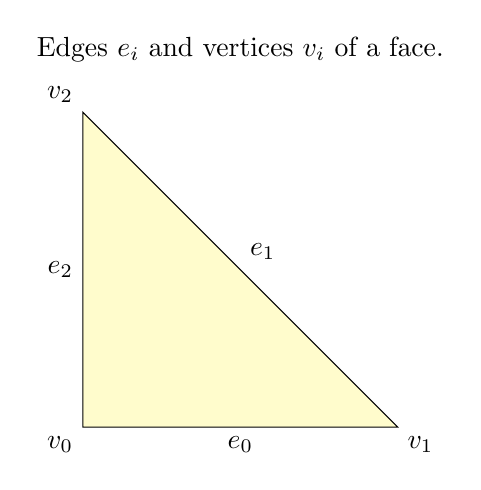
\begin{tikzpicture}[scale=4,wall/.style ={fill=yellow!20!white, draw=black}]
%draw particle 0
\draw (.5,1.2) node {Edges $e_i$ and vertices $v_i$ of a face.};
\draw[wall] (0,0) node[below left]  {$v_0$} 
-- node[midway,below]  {$e_0$}  
(1,0) node[below right]  {$v_1$}
-- node[midway,above right]  {$e_1$}  
(0,1) node[above left]  {$v_2$}
-- node[midway,left]  {$e_2$}  
cycle;
\end{tikzpicture}
\end{document}